\subsection{Oscilloscope}
\markright{Oscilloscope}

\subsubsection*{Definition}
An oscilloscope is an electronic test instrument that displays the variation of an
electrical signal (voltage) as a function of time \cite{wiki:oscilloscope}. It was
first developed in the 1890s as the cathode-ray oscilloscope (CRO), which deflected an
electron beam across a phosphorescent screen. Modern instruments are digital storage
oscilloscopes (DSOs): the analog input is sampled and digitized by an analog-to-digital
converter (ADC), stored in memory, and rendered on an LCD. DSOs can store waveforms for
later analysis, perform automatic measurements, and transfer data to a PC via USB or
LAN.

This laboratory is equipped with three oscilloscope models:

\begin{figure}[H]
  \centering
  \begin{subfigure}[b]{0.31\textwidth}
    \centering
    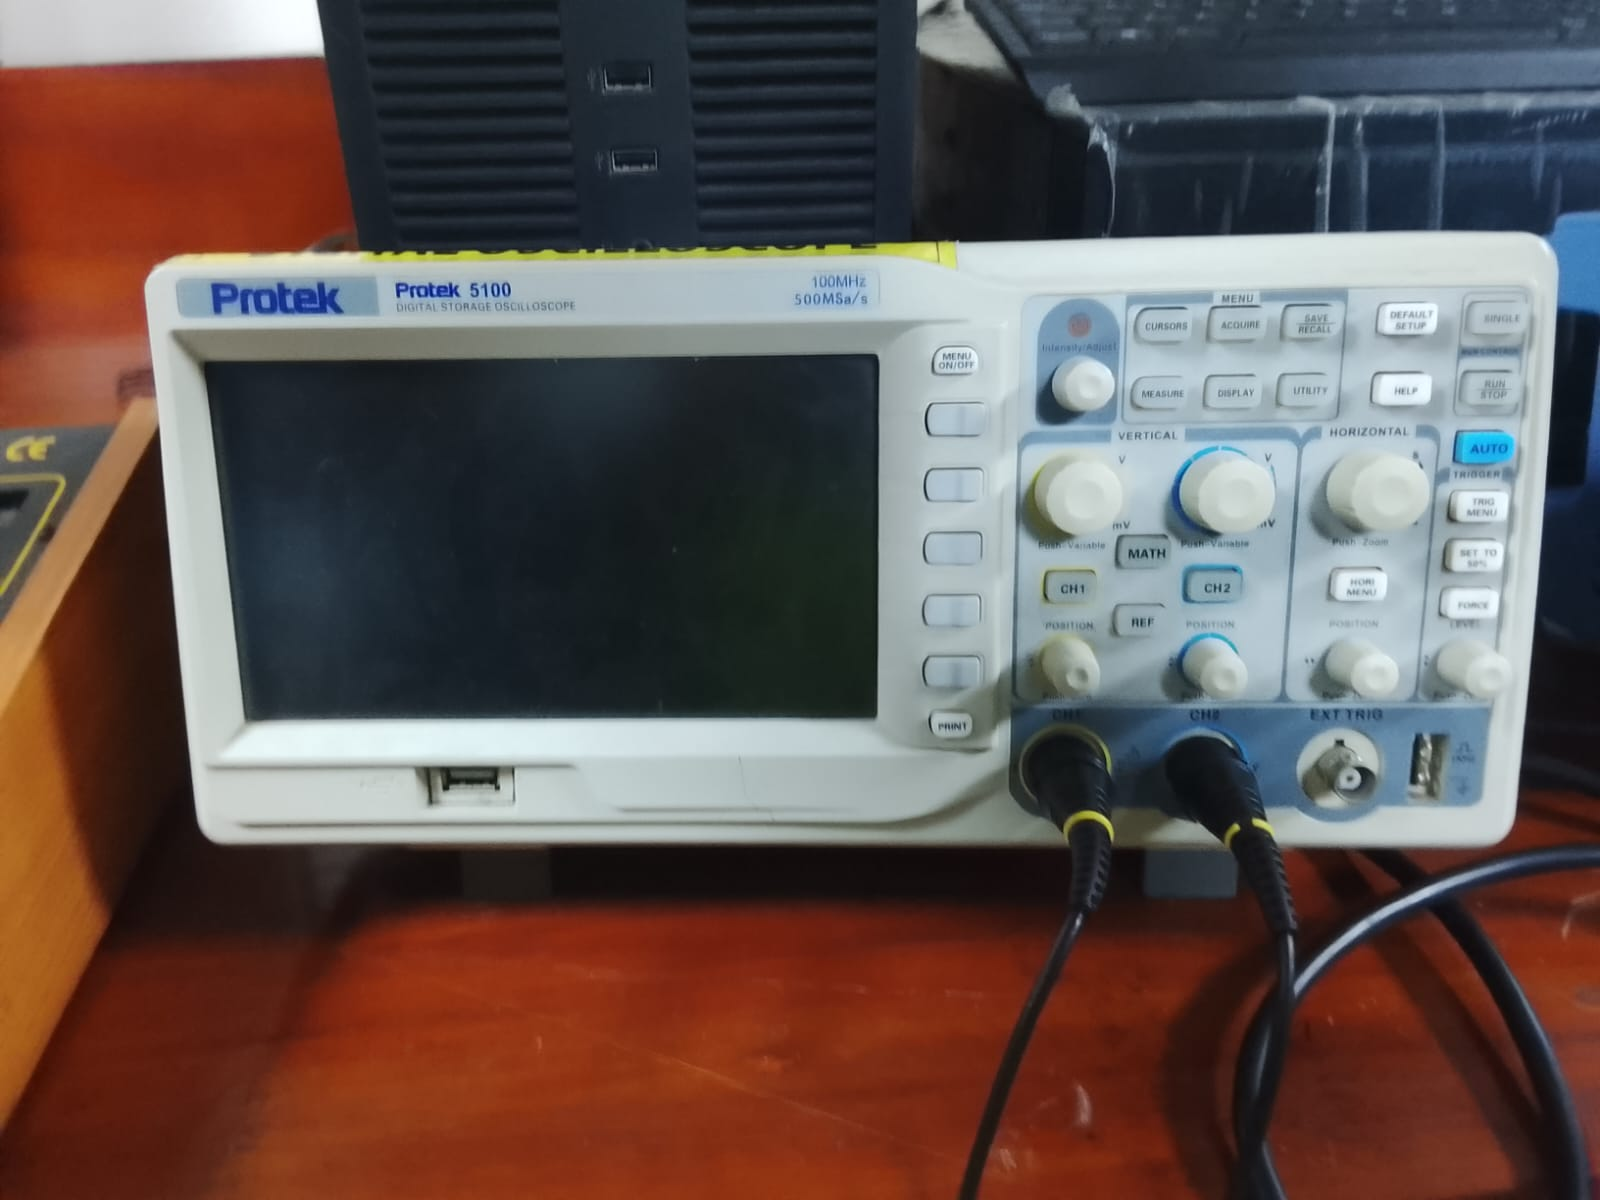
\includegraphics[width=\textwidth, height=4.5cm, keepaspectratio]{lab-01/assets/protek-5100.jpeg}
    \caption{Protek 5100 DSO\\(100\,MHz, 500\,MSa/s)}
  \end{subfigure}
  \hfill
  \begin{subfigure}[b]{0.31\textwidth}
    \centering
    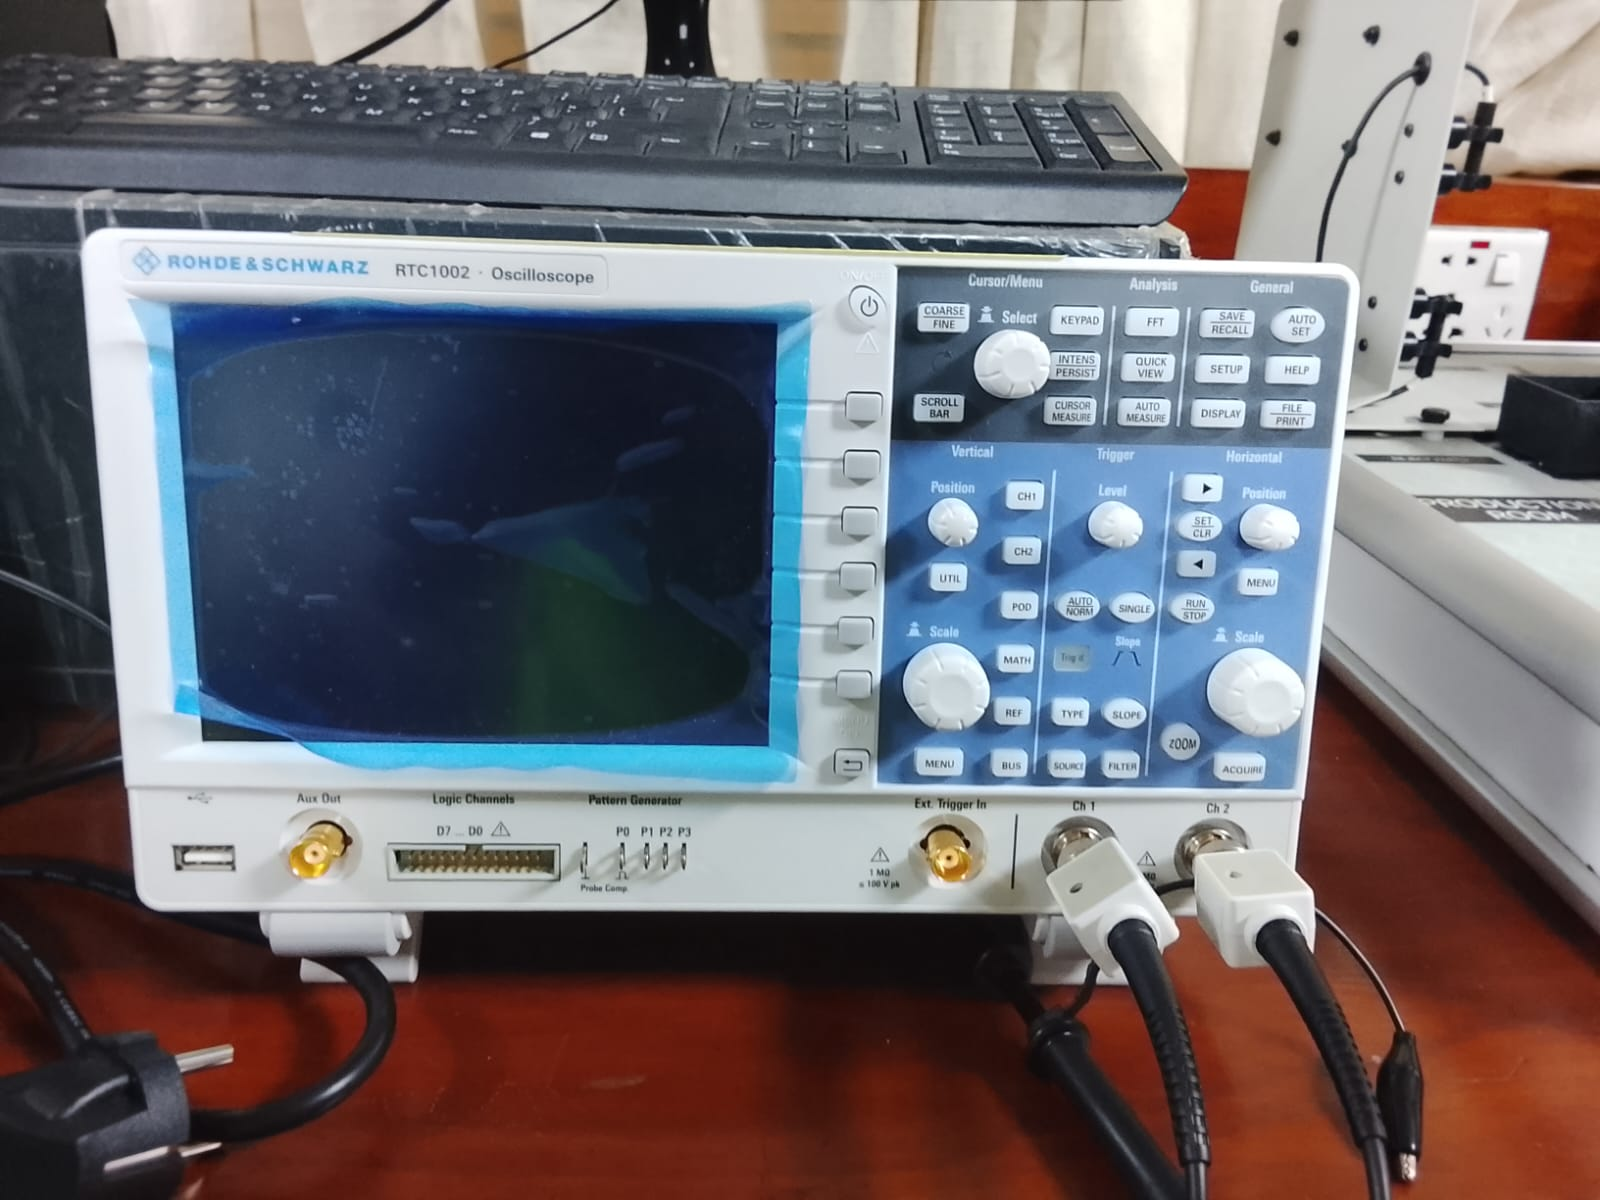
\includegraphics[width=\textwidth, height=4.5cm, keepaspectratio]{lab-01/assets/rs_rtc1002.jpeg}
    \caption{Rohde \& Schwarz RTC1002\\(300\,MHz, 2\,GSa/s)}
  \end{subfigure}
  \hfill
  \begin{subfigure}[b]{0.31\textwidth}
    \centering
    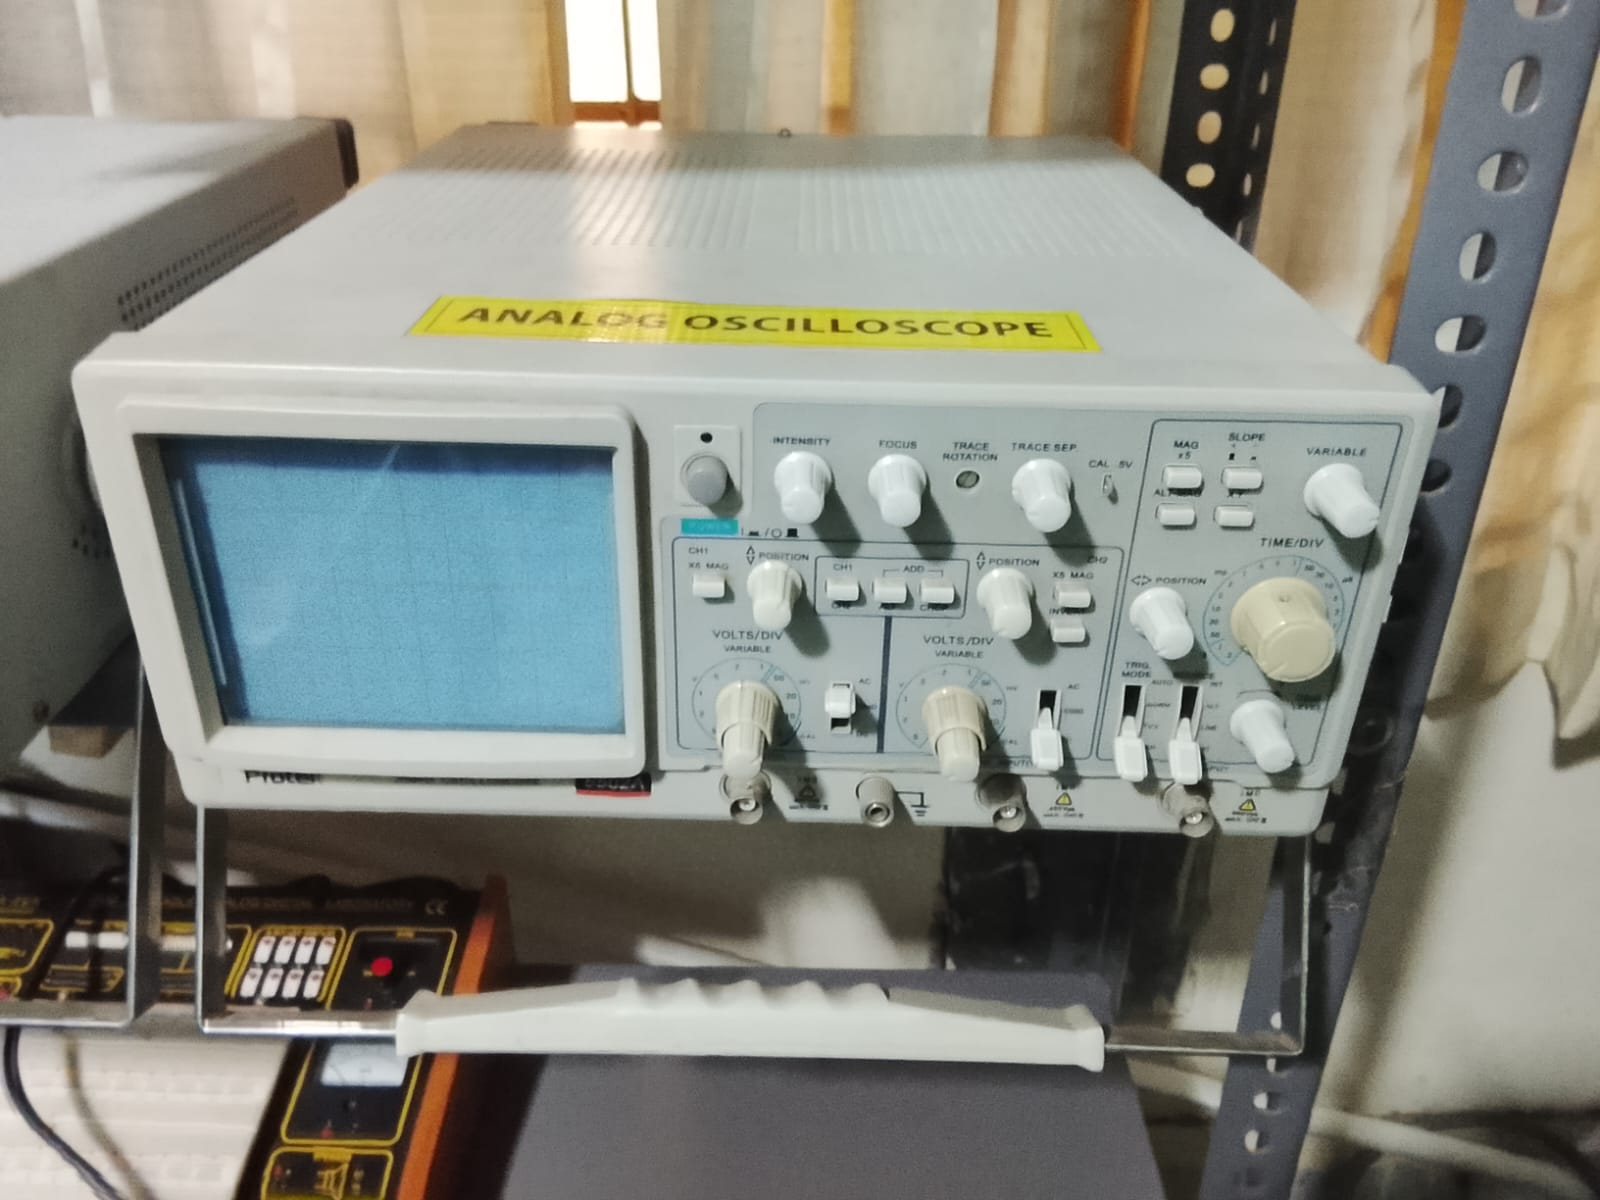
\includegraphics[width=\textwidth, height=4.5cm, keepaspectratio]{lab-01/assets/analog_oscilloscope.jpeg}
    \caption{Analog oscilloscope\\(CRT display)}
  \end{subfigure}
  \caption{Oscilloscopes available in the EEE 2188 laboratory: (a) Protek 5100 DSO,
           (b) Rohde \& Schwarz RTC1002, and (c) analog CRT oscilloscope.}
  \label{fig:oscilloscopes}
\end{figure}

\subsubsection*{Specifications}
The most critical oscilloscope specification is \textit{bandwidth}---the $-3$\,dB
frequency at which a sinusoidal input is attenuated to 70.7\% of its true amplitude
\cite{tek:oscilloscope}. The Protek 5100 in this lab provides 100\,MHz bandwidth and
500\,MSa/s sampling rate; the Rohde \& Schwarz RTC1002 offers 300\,MHz and 2\,GSa/s.
As a rule of thumb, the oscilloscope bandwidth should be at least five times the highest
signal frequency of interest \cite{keysight:bandwidth}. Other key specifications include
vertical sensitivity (typically 1\,mV/div to 10\,V/div), time base
(ns/div to s/div), memory depth, number of channels, and trigger modes (edge, pulse,
video, serial bus).

\subsubsection*{Purpose of Use}
The oscilloscope reveals time-domain waveform information that a multimeter cannot
capture: signal shape, frequency, amplitude, phase, rise time, duty cycle, harmonic
content, and transient events. Two-channel instruments allow the simultaneous display of
input and output signals to measure gain and phase shift.

\subsubsection*{Applications}
Oscilloscopes are used in electronics design, manufacturing test, telecommunications
(signal integrity analysis), power electronics (switching transient measurement in
inverters), automotive diagnostics (CAN/LIN bus decoding), and biomedical engineering
(ECG, EEG signal acquisition) \cite{wiki:oscilloscope}.
